        \clearpage
        \begin{figure*}[ht]
            \pdfbookmark[2]{ID 06}{figure_id_06}
        	\centering
            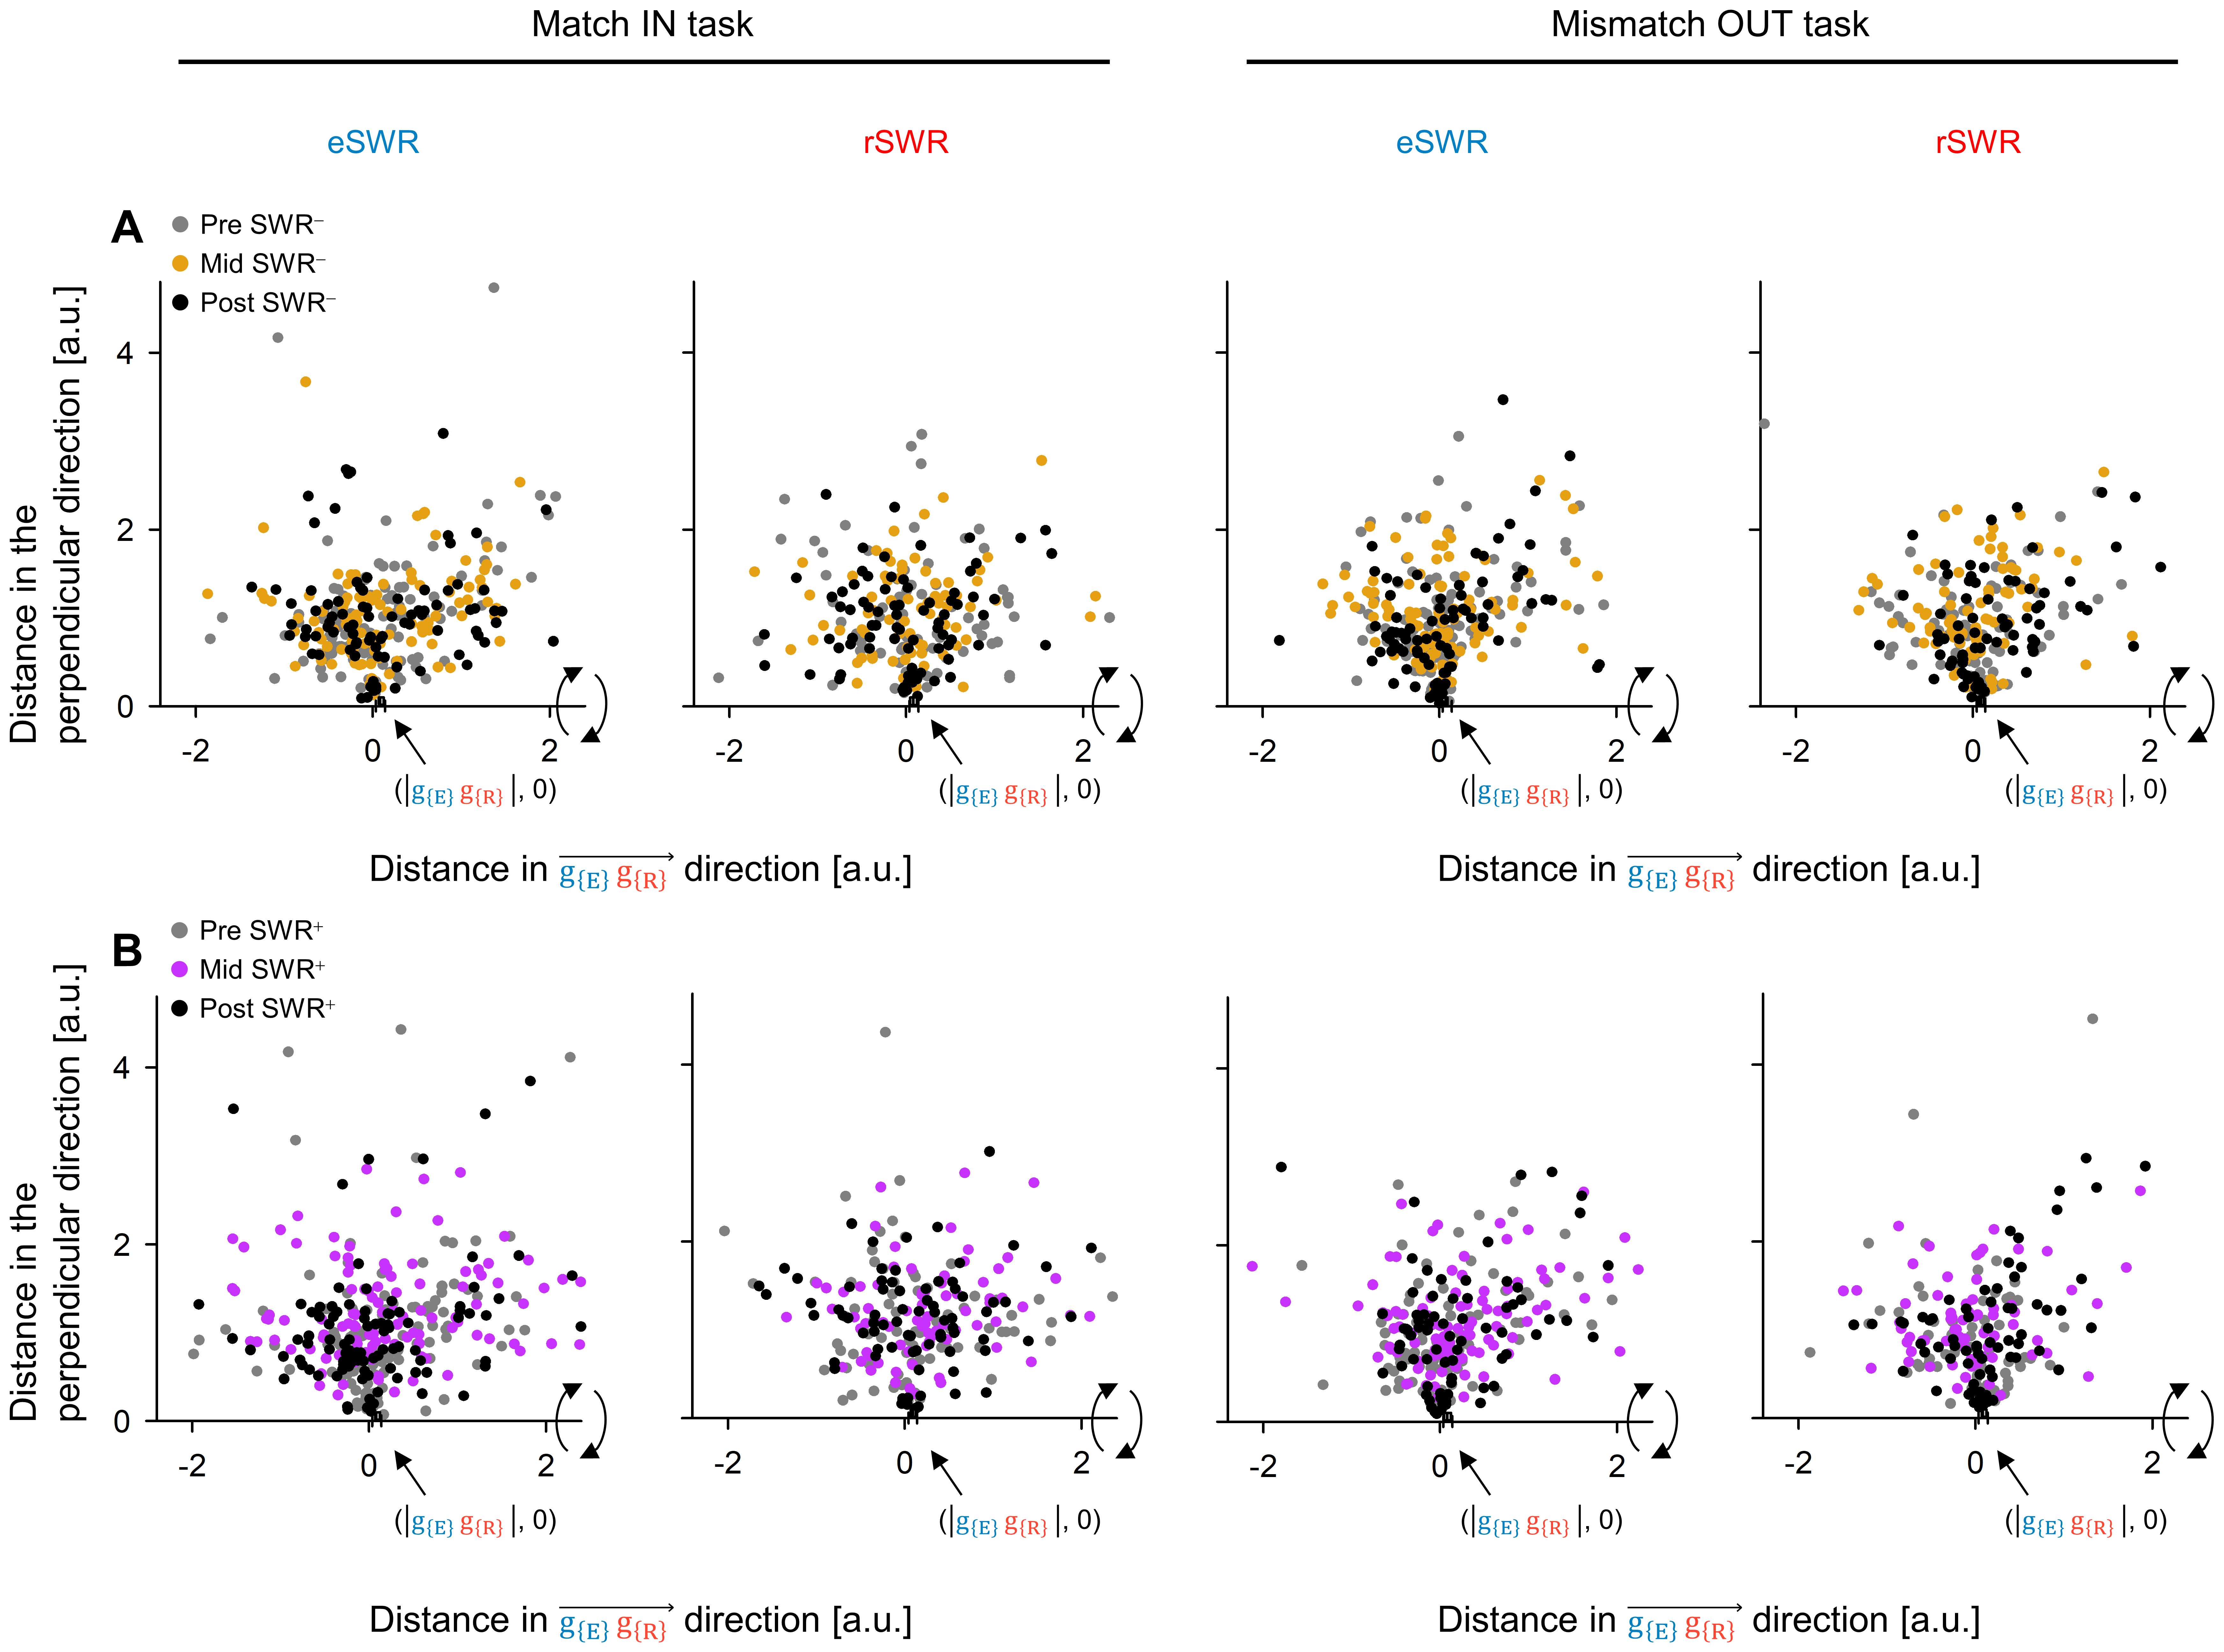
\includegraphics[width=1\textwidth]{./src/figures/.png/Figure_ID_06.png}
        	\caption{\textbf{
Coordinates of neural trajectory during sharp-wave ripple aligned by encoding and retrieval states.
}
\smallskip
\\
\textbf{\textit{A.}} Hippocampal neural trajectories during pre- (\textit{gray}), mid- (\textit{yellow}), and post-SWR$^-$ (\textit{black}) in Match IN (\textit{left}) and Mismatch OUT task (\textit{right}). \textbf{\textit{B.}} The equivalents for SWR$^+$ instead of SWR$^-$, though mid-SWR$^+$ is depicted with \textit{purple}. All data points underwent adjustments and rotations to fit a two-dimensional representation, positioning $\mathrm{g_{E}}$ at (0, 0) and $\mathrm{g_{R}}$ at ($\lVert \mathrm{g_{E}g_{R}} \rVert$, 0). The $\lVert \mathrm{g_{E}g_{R}} \rVert$ metric varies across sessions, and its median \textpm IQR (with medians approximately 0.2) is presented on the x-axes. Note: some intervals might be challenging to discern because of their narrow range. In this two-dimensional depiction, both the distances and angles preserve their relationships as in the original three-dimensional space. Abbreviations: SWR, sharp-wave ripple events; eSWR, SWR during the encoding phase; rSWR, SWR during the retrieval phase, SWR$^+$, SWR event; SWR$^-$ control events for SWR$^+$; pre-SWR, mid-SWR, or post-SWR, the time interval from $-800$ to $-250$ ms, from $-250$ to $+250$ ms, or from $+250$ to $+800$ ms from the center of SWR.
}
% width=1\textwidth
        	\label{fig:06}
        \end{figure*}
